\subsection{Value chain}


Porter's value chain model beskriver et firma ud fra de aktiviteter der skal udføres for at tilføje værdi til de "rå" materialer.
Eftersom modellen er konstrueret med konventionelle fremstillingsvirksomheder i tankerne kan det ikke direkte overføres til softwarevirksomheder.
Softwarevirksomheder indkøber sjældent rå materialer i traditionel forstand, men ideerne gælder stadig på et konceptuelt niveau.

Følgendende beskrivelse er baseret på \citet[p.~12]{rose2012software}.

Aktiviteter inddeles i to kategorier, de primære og support aktiviteter.
De primære aktiviteter beskriver hvordan virksomheden omdanner rå materialer til det færdige produkt på hylden ved at tilføje værdi.
Support aktiviteterne bidrager til denne omdannelse uden direkte at tilføre værdi, dette kan eksempelvis være research.
Modellen er illustreret på  \cref{valuechain}.

\begin{figure}
	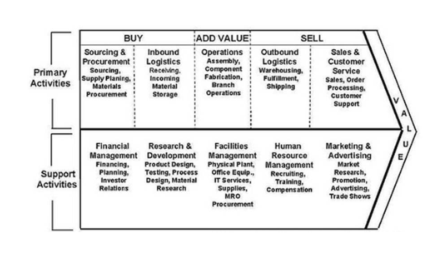
\includegraphics[width=\textwidth]{valuechain.PNG}
	\caption{Porters valuechain model}
	\label{valuechain}
\end{figure}

\paragraph{Model af SharePass}
Følgende er en valuechain model af SharePass virksomheden.
De primære aktiviteter består i at indkøbe de hardwaredele som vi ikke selv kan stå for at producere.
Vi tilføjer derefter værdi til disse ved at designe sikkerhedsprotokoller til enhederne samt software til klient og server.
Værdien består primært i at lave en løsning der virker med et minimum af interaktion men stadig sikkert.
Salgsdelen går derefter ud på at sælge produktet til virksomheder og derefter yde support så de får mest muligt ud af produktet.

Til at muliggøre de primære aktiviteter benyttes supportaktiviteterne.
For at sikre den højst mulige sikkerhed er det nødvendigt at hyre eksperter i sikkerhed.
Ligeledes har vi brug for ekspertise inden for udvikling af hardwaredelen af produktet.
Der skal derfor også hyres eksperter inden for elektronik og hardware samt koblingen mellem elektronikken og software systemet.
For at få produktet solgt er det vigtigt at henvende sig til virksomheder på en måde der kan overbevise dem om hvorvidt de har et behov for produktet.
Til dette skal der bruges en marketingafdeling

\todo{skal itemize forblive her? Figur?}
\subsubsection*{Primære aktiviteter}
Køb:
\begin{itemize}
\item NFC kort
\item Fysisk login med NFC kort hos firma - her opdateres passwords på kortet
\end{itemize}
Tilføj værdi:
\begin{itemize}
\item Sikkerhedsprotokol mellem fysisk login portal og server
\item Sikkerhedsprotokol mellem klient og NFC kort
\item Sikkerhedsprotokol mellem fysisk login portal og NFC kort
\item Software til password server
\item Software til klient
\end{itemize}
Sælg:
\begin{itemize}
\item Sælg produkt som pakke
\item Tilbyd support
\end{itemize}

\subsubsection*{Support aktiviteter}
\begin{itemize}
\item Marketing
\item Hyre - sikkerhedsekspert, hardwaredesigner
\end{itemize}